    
%% Beginning of file 'sample63.tex'
%%
%% Modified 2019 June
%%
%% This is a sample manuscript marked up using the
%% AASTeX v6.3 LaTeX 2e macros.
%%
%% AASTeX is now based on Alexey Vikhlinin's emulateapj.cls 
%% (Copyright 2000-2015).  See the classfile for details.

%% AASTeX requires revtex4-1.cls (http://publish.aps.org/revtex4/) and
%% other external packages (latexsym, graphicx, amssymb, longtable, and epsf).
%% All of these external packages should already be present in the modern TeX 
%% distributions.  If not they can also be obtained at www.ctan.org.

%% The first piece of markup in an AASTeX v6.x document is the \documentclass %%
%% command. LaTeX will ignore any data that comes before this command. The 
%% documentclass can take an optional argument to modify the output style.
%% The command below calls the preprint style which will produce a tightly 
%% typeset, one-column, single-spaced document.  It is the default and thus
%% does not need to be explicitly stated.
%%
%%
%% using aastex version 6.3
\documentclass[twocolumn]{aastex63}

%% The default is a single spaced, 67 point font, single spaced article.
%% There are 5 other style options available via an optional argument. They
%% can be invoked like this:
%%
% \documentclass[arguments]{aastex63}
%% 
%% where the layout options are:
%%
%%  twocolumn   : two text columns, 10 point font, single spaced article.
%%                This is the most compact and represent the final published
%%                derived PDF copy of the accepted manuscript from the publisher
%%  manuscript  : one text column, 12 point font, double spaced article.
%%  preprint    : one text column, 12 point font, single spaced article.  
%%  preprint2   : two text columns, 12 point font, single spaced article.
%%  modern      : a stylish, single text column, 12 point font, article with
%% 		  wider left and right margins. This uses the Daniel
%% 		  Foreman-Mackey and David Hogg design.
%%  RNAAS       : Preferred style for Research Notes which are by design 
%%                lacking an abstract and brief. DO NOT use \begin{abstract}
%%                and \end{abstract} with this style.
%%
%% Note that you can submit to the AAS Journals in any of these 6 styles.
%%
%% There are other optional arguments one can invoke to allow other stylistic
%% actions. The available options are:
%%
%%   astrosymb    : Loads Astrosymb font and define \astrocommands. 
%%   tighten      : Makes baselineskip slightly smaller, only works with 
%%                  the twocolumn substyle.
%%   times        : uses times font instead of the default
%%   linenumbers  : turn on lineno package.
%%   trackchanges : required to see the revision mark up and print its output
%%   longauthor   : Do not use the more compressed footnote style (default) for 
%%                  the author/collaboration/affiliations. Instead print all
%%                  affiliation information after each name. Creates a much 
%%                  longer author list but may be desirable for short 
%%                  author papers.
%% twocolappendix : make 2 column appendix.
%%   anonymous    : Do not show the authors, affiliations and acknowledgments 
%%                  for dual anonymous review.
%%
%% these can be used in any combination, e.g.
%%
%% \documentclass[twocolumn,linenumbers,trackchanges]{aastex63}
%%
%% AASTeX v6.* now includes \hyperref support. While we have built in specific
%% defaults into the classfile you can manually override them with the
%% \hypersetup command. For example,
%%
%% \hypersetup{linkcolor=red,citecolor=green,filecolor=cyan,urlcolor=magenta}
%%
%% will change the color of the internal links to red, the links to the
%% bibliography to green, the file links to cyan, and the external links to
%% magenta. Additional information on \hyperref options can be found here:
%% https://www.tug.org/applications/hyperref/manual.html\#x1-40003
%%
%% Note that in v6.3 "bookmarks" has been changed to "true" in hyperref
%% to improve the accessibility of the compiled pdf file.
%%
%% If you want to create your own macros, you can do so
%% using \newcommand. Your macros should appear before
%% the \begin{document} command.
%%
\newcommand{\vdag}{(v)^\dagger}
\newcommand\aastex{AAS\TeX}
\newcommand\latex{La\TeX}

\date{\today}

% \accepted{\today}
%% Command to document which AAS Journal the manuscript was submitted to.
%% Adds "Submitted to " the argument.
% \submitjournal{AJ}

%% For manuscript that include authors in collaborations, AASTeX v6.3
%% builds on the \collaboration command to allow greater freedom to 
%% keep the traditional author+affiliation information but only show
%% subsets. The \collaboration command now must appear AFTER the group
%% of authors in the collaboration and it takes TWO arguments. The last
%% is still the collaboration identifier. The text given in this
%% argument is what will be shown in the manuscript. The first argument
%% is the number of author above the \collaboration command to show with
%% the collaboration text. If there are authors that are not part of any
%% collaboration the \nocollaboration command is used. This command takes
%% one argument which is also the number of authors above to show. A
%% dashed line is shown to indicate no collaboration. This example manuscript
%% shows how these commands work to display specific set of authors 
%% on the front page.
%%
%% For manuscript without any need to use \collaboration the 
%% \AuthorCollaborationLimit command from v6.2 can still be used to 
%% show a subset of authors.
%
%\AuthorCollaborationLimit=2
%
%% will only show Schwarz & Muench on the front page of the manuscript
%% (assuming the \collaboration and \nocollaboration commands are
%% commented out).
%%
%% Note that all of the author will be shown in the published article.
%% This feature is meant to be used prior to acceptance to make the
%% front end of a long author article more manageable. Please do not use
%% this functionality for manuscripts with less than 20 authors. Conversely,
%% please do use this when the number of authors exceeds 40.
%%
%% Use \textit{all}authors at the manuscript end to show the full author list.
%% This command should only be used with \AuthorCollaborationLimit is used.

%% The following command can be used to set the latex table counters.  It
%% is needed in this document because it uses a mix of latex tabular and
%% AASTeX deluxetables.  In general it should not be needed.
%\setcounter{table}{1}

%%%%%%%%%%%%%%%%%%%%%%%%%%%%%%%%%%%%%%%%%%%%%%%%%%%%%%%%%%%%%%%%%%%%%%%%%%%%%%%%
%%
%% The following section outlines numerous optional output that
%% can be displayed in the front matter or as running meta-data.
%%
%% If you wish, you may supply running head information, although
%% this information may be modified by the editorial offices.
\shorttitle{Cluster Eclipsing Binaries}
\shortauthors{Bowen \& Geller}
%%
%% You can add a light gray and diagonal water-mark to the first page 
%% with this command:
%% \watermark{text}
%% where "text", e.g. DRAFT, is the text to appear.  If the text is 
%% long you can control the water-mark size with:
%% \setwatermarkfontsize{dimension}
%% where dimension is any recognized LaTeX dimension, e.g. pt, in, etc.
%%
%%%%%%%%%%%%%%%%%%%%%%%%%%%%%%%%%%%%%%%%%%%%%%%%%%%%%%%%%%%%%%%%%%%%%%%%%%%%%%%%
\graphicspath{{./}{figures/}}
%% This is the end of the preamble.  Indicate the beginning of the
%% manuscript itself with \begin{document}.

% \usepackage{siunitx}
% \usepackage{caption}
% \usepackage{subcaption}
% \captionsetup{compatibility=false}
\usepackage{graphicx}
\usepackage{appendix}
\usepackage{savesym}
\savesymbol{tablenum}
\usepackage{morefloats}
\usepackage{subfigure}
% \usepackage[showframe]{geometry}% http://ctan.org/pkg/geometry


\begin{document}


\title{Simulating the Period-Recovery Yield of Eclipsing Binaries in Star Clusters with LSST}

%% LaTeX will automatically break titles if they run longer than
%% one line. However, you may use \\ to force a line break if
%% you desire. In v6.3 you can include a footnote in the title.

%% A significant change from earlier AASTEX versions is in the structure for 
%% calling author and affiliations. The change was necessary to implement 
%% auto-indexing of affiliations which prior was a manual process that could 
%% easily be tedious in large author manuscripts.
%%
%% The \author command is the same as before except it now takes an optional
%% argument which is the 16 digit ORCID. The syntax is:
%% \author[xxxx-xxxx-xxxx-xxxx]{Author Name}
%%
%% This will hyperlink the author name to the author's ORCID page. Note that
%% during compilation, LaTeX will do some limited checking of the format of
%% the ID to make sure it is valid. If the "orcid-ID.png" image file is 
%% present or in the LaTeX pathway, the OrcID icon will appear next to
%% the authors name.
%%
%% Use \affiliation for affiliation information. The old \affil is now aliased
%% to \affiliation. AASTeX v6.3 will automatically index these in the header.
%% When a duplicate is found its index will be the same as its previous entry.
%%
%% Note that \altaffilmark and \altaffiltext have been removed and thus 
%% can not be used to document secondary affiliations. If they are used latex
%% will issue a specific error message and quit. Please use multiple 
%% \affiliation calls for to document more than one affiliation.
%%
%% The new \altaffiliation can be used to indicate some secondary information
%% such as fellowships. This command produces a non-numeric footnote that is
%% set away from the numeric \affiliation footnotes.  NOTE that if an
%% \altaffiliation command is used it must come BEFORE the \affiliation call,
%% right after the \author command, in order to place the footnotes in
%% the proper location.
%%
%% Use \email to set provide email addresses. Each \email will appear on its
%% own line so you can put multiple email address in one \email call. A new
%% \correspondingauthor command is available in V6.3 to identify the
%% corresponding author of the manuscript. It is the author's responsibility
%% to make sure this name is also in the author list.
%%
%% While authors can be grouped inside the same \author and \affiliation
%% commands it is better to have a single author for each. This allows for
%% one to exploit all the new benefits and should make book-keeping easier.
%%
%% If done correctly the peer review system will be able to
%% automatically put the author and affiliation information from the manuscript
%% and save the corresponding author the trouble of entering it by hand.

% Authors & affiliations
\email{andrewbowen2020@u.northwestern.edu\\
a-geller@northwestern.edu}

% Andrew's stuff
\author{Andrew Bowen}
\affiliation{
Center for Interdisciplinary Exploration and Research in Astrophysics, 1800 Sherman Ave, 8th Floor
Northwestern University, CIERA Evanston, IL 60201
}

% Aaron's stuff
\author{Aaron M. Geller}

\affiliation{Adler Planetarium, 1300 S Lake Shore Dr, Chicago, IL 60605
}
\altaffiliation{Center for Interdisciplinary Exploration and Research in Astrophysics, 1800 Sherman Ave, 8th Floor
Northwestern University, CIERA Evanston, IL 60201}

%% Note that the \and command from previous versions of AASTeX is now
%% depreciated in this version as it is no longer necessary. AASTeX 
%% automatically takes care of all commas and "and"s between authors names.

%% AASTeX 6.3 has the new \collaboration and \nocollaboration commands to
%% provide the collaboration status of a group of authors. These commands 
%% can be used either before or after the list of corresponding authors. The
%% argument for \collaboration is the collaboration identifier. Authors are
%% encouraged to surround collaboration identifiers with ()s. The 
%% \nocollaboration command takes no argument and exists to indicate that
%% the nearby authors are not part of surrounding collaborations.

% Abstract - used at AAS, updated slightly
\begin{abstract}
We present a study of the period-recovery capability of the Large Synoptic Survey Telescope (LSST) for eclipsing binary stars in star clusters. Unlike binaries in the galactic field, dynamical encounters within the dense environment of a star cluster can modify the orbital parameters of binaries stars, by changing the periods and eccentricities and exchanging in different companions. Therefore, eclipsing binaries in star clusters may allow for insights into both the intrinsic properties of the binary’s component stars, as well as the dynamical histories of the binary population. For our simulations, we use \texttt{COSMIC} to generate and evolve populations of binaries specifically catered to each of the thousands of galactic open and globular clusters (e.g., matching the cluster ages, metallicities, periods at the hard-soft boundary, etc.). We generate simulated light curves, using the LSST filters and expected cadence and accounting for the expected photometric precision of LSST, for each observable eclipsing binary, using the \texttt{ellc} code. We then attempt to recover the orbital period for each observed binary through a Lomb-Scargle periodogram, using \texttt{gatspy} software. We compare the \textit{baseline} cadence proposed for LSST to a \textit{colossus} cadence that samples the galactic plane (where most open clusters reside) more evenly. In this paper, we present expected recovery statistics for eclipsing binary stars in the galactic open and globular star clusters for both of these proposed observing strategies. In addition, we discuss potential eclipsing White Dwarf binary systems that will be detectable by both LSST in the visible band and the Laser Interferometer Space Antenna (LISA) in gravitational waves.  Overall, for cluster-member eclipsing binaries, the \textit{colossus} plan proves more robust for effective period-recovery.

\end{abstract}

\keywords{LSST -- eclipsing binaries}

%%%%%%% -------------------------------------------------------------------------------------------------------------------

%%% Introduction %%%
\section{Introduction} \label{sec:Intro}
When the \textit{Large Synoptic Survey Telescope} (LSST) becomes operational in 2021, it will provide unprecedented data on eclipsing binary stars (EBs). Different attempts to find the period recovery rate for LSST in terms of eclipsing binary stars have been made by \citet{2011AJ....142...52P} and more recently in \citet{2017PASP..129f5003W} and \citet{2019AAS...23336317P}. We attempt to build on previous work by including eclipsing binary stars residing in open and globular clusters. Given that nearly half of all stars within the Milky Way reside in a binary system, and a significant number also reside in star clusters, these cluster binaries make up an important population of all galactic EBs. 

% Data compilation and refs
We compiled data for open clusters from \citet{2008A&A...477..165P}, \citet{2004A&A...414..163S}, \citet{2006AJ....131.1559V}, and the WEBDA catalog \citep{1995MNRAS.275..828M}, alongside globular cluster data by \citet{1996AJ....112.1487H}. 

% Binary encounters
The behavior of binary stars bound in clusters can be different than those binaries distributed throughout the rest of the galaxy because of close gravitational encounters with nearby stars. The higher rate of close stellar encounters within star clusters could influence the recovery rate for EBs within clusters. We account for intra-cluster binary encounters discussed in \citet{2015ApJ...808L..25G}. A hard-soft period limit (Equation~\ref{eq: hs-boundary}) is imposed on binaries generated by the population-synthesis software used. We use \texttt{COSMIC} \citep{2018PhDT........74B} to evolve populations of binary stars for every open and globular cluster. Light curve generation software \texttt{ellc}, created by \citet{2016ascl.soft03016M} allows us to create light curves able to be fit and phase-folded by \texttt{gatspy} \citep{2015ApJ...812...18V}. The light curves are then passed to a Lomb-Scargle (LS) periodogram in order to recover the period from an observed light curve. The recovered period from our light curve analysis is checked against the ‘input period’ initiated from COSMIC for a test of accuracy of our method.

% WD binary theory
Detached White Dwarf (DWD) binary stars are a particularly interesting sub-section of binary systems that will be detectable by both LSST via observed eclipses and the \textit{Laser Interferometer Space Antenna} (LISA) via gravitational waves (GW). DWD binaries with periods $p \leq 0.1 days$ will have large enough GW strain to be detected by LISA \citep{2017MNRAS.470.1894K}. The possibility of a detection overlap  an eclipsing white dwarf (WD) binary system by both LSST and LISA have been studied in \citet{2017MNRAS.470.1894K}. However, we extend this analysis to include period recovery in addition to sole detection of DWD eclipses. We also will analyze DWDs within our sample in addition to other binaries. Observing WD binaries with both electromagnetic radiation and gravitational wave detectors provides an important step in the development of multi-messenger astronomy.

% Paper layout
The remainder of this paper is laid out as follows. In Section~\ref{sec:Methods} we discusss our method for simulation and analysis of EB light curves in star clusters. In Section~\ref{sec:Results} we describe the results of our cluster binary population simulations. Section~\ref{sec:Conclusion} gives wider implications of our results.
Appendix~\ref{app:Appendix A} includes relevant plots and figures.

%%%%%%%%----------------------------------------------------------------------

%%% Methods %%%
\section{Methods} \label{sec:Methods}

% Compiling Cluster Dataframes
\subsection{Cluster Data} \label{sec:compiling}

We first compiled cluster data for 157 globular clusters (GCs) and 3353 open clusters (OC). The GC data was compiled from tables provided by \citet{1996AJ....112.1487H}. These tables include cluster coordinates (RA/Dec), metallicities, velocity dispersions (km/s), ages (Myr), and distances (kpc). For the OCs, we compiled data from several databases, including the WEBDA database \citet{1995MNRAS.275..828M}, \citet{2013A&A...558A..53K}, \citet{2004A&A...414..163S}, and \citet{2008A&A...477..165P}. These databases used inconsistent units, so corrections were made to standardize both database labels as well as to convert units across all tables. The cluster parameters listed above were needed for our algorithm to run properly.

% OpSim Overlap and Strategies
\subsection{Cluster Viewing Fields} \label{sec:overlap}
We make use of the Operations Simulator (hereafter \textit{OpSim}) to simulate LSST observation. We utilize both the \textit{baseline} and \textit{colossus}\footnote{It should be noted that there are several \textit{colossus} observing strategies for LSST. The strategy used in this paper corresponds to the 'colossus-2664' MySQL data file, which weighs the galactic plane more heavily in terms of $N_{obs}$} viewing strategies in an effort to compare effectiveness of recovering EB periods (see Figures~\ref{fig:cluster_mollweide}~and~ \ref{fig:baseline_mollweide}). 
% Some clusters’ on-sky locations will overlap with multiple LSST viewing fields (\ref{fig:cluster_mollweide} and \ref{fig:baseline_mollweide}.

% Mollweides of Clusters and strategies
\begin{figure}
    \centering
    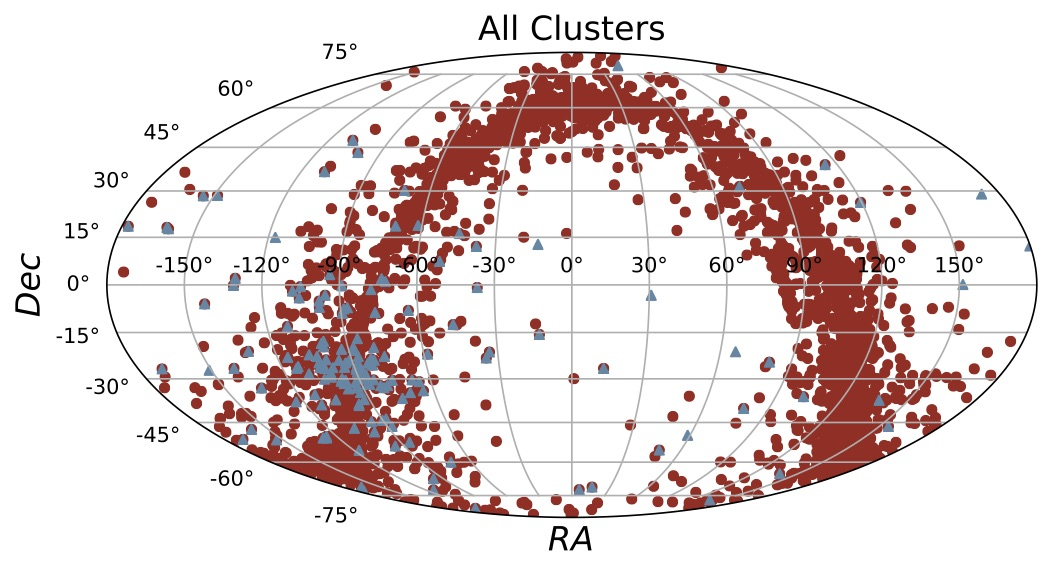
\includegraphics[width=0.4\textwidth]{figures/mollweides/clusters-opsim-mollweide.pdf}
    \caption{Mollweide projection plot of open clusters (red) along with globular clusters (blue) plotted in their on-sky locations. These locations are significant in that they vary in Nobs under different LSST observing strategies.}
    \label{fig:cluster_mollweide}
\end{figure}

\begin{figure}
    \centering
    % Baseline molleweide
        \includegraphics[width=0.4\textwidth]{figures/mollweides/baseline-Nobs-mollweide.pdf}
    % Colossus molleweide
        \includegraphics[width=0.4\textwidth]{figures/mollweides/colossus-Nobs-mollweide.pdf}
        
        \caption{Mollweide projection plot of Number of observations per OpSim field, $N_{obs}$, values for each \textit{OpSim} viewing field for \textit{baseline} (top) and \textit{colossus} (bottom) at each \textit{OpSim} viewing field. The colossus strategy more heavily weighs the galactic plane in terms of $N_{obs}$, which is where a considerable number of both GCs and OCs reside in terms of on-sky location (see \ref{fig:cluster_mollweide}).}
        \label{fig:colossus_mollweide}
        \label{fig:baseline_mollweide}

\end{figure}

% Multiple overlaps & OpSim cadence
We took into consideration clusters that overlapped with more than one \textit{OpSim} field. This could alter the period recovery for EBs within that cluster due to a different $N_{obs}$. Across all \textit{OpSim} fields, 29.3\% of GCs and 33.5\% of OCs overlap with more than 1 \textit{OpSim} fields. On the other hand, 24.2\% of OCs and 23.7\% of GCs overlapped with more than 1 \textit{OpSim} field with $N_{obs} > 0$ for \textit{baseline}. Because the fraction of clusters that overlap with multiple OpSim fields is small, we consider the closest on-sky neighbor field to be the closest field for each cluster. Consequently, the cadence used for each cluster is designated by its nearest on-sky neighbor.

% Strategy comparison -- why colossus is better
Our objective is to compare the proposed \textit{OpSim} observing strategies \textit{baseline} and \textit{colossus}. \textit{Colossus} generally allocates higher $N_{obs}$ values for viewing fields in and around the galactic plane. This could result in a higher yield of \textit{recovered} binaries in OCs specifically because of their location throughout the galactic plane, whereas GCs reside primarily in a spherical distribution centered on the galactic center (see \ref{fig:cluster_mollweide}). Due to the line-of-sight to some of these GCs being in \textit{OpSim} fields where \textit{colossus} has higher $N_{obs}$ values than \textit{baseline}, it is feasible that GCs could potentially have higher period recovery with \textit{colossus as well}. Due to different weighing of observation rates of the galactic plane, \textit{colossus} could potentially recovery higher rates of field EBs as well.


% COSMIC Simulation - figure out citing protocol for software
% COSMIC Docs: https://cosmic-popsynth.github.io/docs/latest/
\subsection{Binary Population Synthesis} \label{subsec:cosmic}
We use COSMIC \citet{2018PhDT........74B} to generate and evolve populations of $N_{*}$ = $4 x 10^4$ binaries to the age of the cluster listed in our compiled cluster data. While $4 x 10^4$ binaries per cluster is not physically representative of the $N_{*}$ in real clusters, we chose this number to have a large enough statistical sample. After simulating a population for each cluster, we also normalize the sample by the true number of binaries in  each cluster. 

We impose a long-period limit on each binary generated by COSMIC, such that the period is below the hard-soft period boundary, \textit{$P_{hs}$} for binaries in star clusters described by \citet{2015ApJ...808L..25G}:

\begin{equation} \label{eq: hs-boundary}
    P_{hs} = \frac{\pi G}{\sqrt{2}} \left( \frac{m_1m_2}{m_3} \right) ^{3/2}(m_1 + m_2)^{-1/2}\sigma_0^{-3}
\end{equation}

% Velocity dispersions
Where $\sigma$ is the cluster velocity dispersion. ‘Hard’ binaries have periods shorter than that of the hard-soft boundary of the cluster. ‘Soft’ binaries have longer periods than that of the boundary, and are most easily disrupted by intra-cluster close binary encounters. This was considered because the distance scales between objects is smaller in star clusters than in the field of the galaxy. Thus, binaries in star clusters will have higher encounter rates than those binaries in the galactic field. Cluster velocity dispersion values were listed for 66 GCs in \citet{1996AJ....112.1487H}. For open clusters, and those globular clusters with no $\sigma$ listed in our catalog, we calculate the projected velocity dispersion\footnote{It should be noted that the $\sigma_0$ in Eq~\ref{eq: hs-boundary} represents the three-dimensional velocity dispersion of a cluster}, $\sigma$  via the half-mass radius, $R_h$, or core radius $R_c$ and cluster mass, $M_cl$, from the Plummer model given in \cite{1911MNRAS..71..460P}:

% Plummer velocity dispersion model
\begin{equation}
    \sigma_z^2 = \frac{3\pi}{64}\frac{GM_{cl}}{r_p}\left(1 + \frac{d^2}{r_p^2} \right)^{-1/2}
    \label{eq:plummer-sigma model}
\end{equation}

 Where $r_p$ is the Plummer scale radius of the cluster \citep{1911MNRAS..71..460P}. This is calculated via $R_h$. However, we assume $d=0$ which reduces Eq~\ref{eq:plummer-sigma model} to:
 
%  Simplified Plummer model
 \begin{equation}
    \sigma_z^2 = \frac{3\pi}{64}\frac{GM_{cl}}{r_p}
    \label{eq:plummer-sigma mode (simplified)l}
\end{equation}
 
 Most parameters are listed in our compiled cluster catalogs for both GCs and OCs. The parameters required from each cluster required for our algorithm to run properly are:
 
%  List of requisite cluster params
\begin{itemize}
    \item Age ($Myr$)
    \item Mass ($M_{\odot}$)
    \item Velocity Dispersion ($km/s$)
    \item Half-mass radius ($R_{\odot}$)
    \item Metallicity
    \item Distance ($kpc$)
\end{itemize}
 For those clusters with parameters  not listed in the literature, we assumed the cluster parameter to be that of the mean value for that parameter among either OCs or GCs. We then use these cluster-specific values as inputs within \texttt{COSMIC} to evolve the binary population to the cluster age.
 
%  Ellc light curve stuff
\subsection{Light Curve Generation}
\label{subsec:ellc}
 We utilize \texttt{ellc} \citep{2016ascl.soft03016M} to generate a theoretical light curve for each binary in the cluster population. The evolved binary parameters from \texttt{COSMIC} were used by \texttt{ellc} as inputs to generate light curves.
 
%  \subsection{Light Curves and the Effects of Crowding on Period Recovery}
One consideration that must be taken in the analysis of EBs in star clusters is the effect of crowding. Either background or foreground objects can contribute additional flux, thus producing the effect of crowding the LSST viewing field. This additional flux could potentially impact the period recovery of EBs when passing the folded and fitted light curves to LS, as shown in Figure~\ref{fig:light3curve}. We model this background flux by using the third-light parameter from \texttt{ellc}.
 
 We use \texttt{gatspy} to generate a fit for the phase-folded light curves across all filters \citep{2016ascl.soft10007V}. The light curves are passed through a Lomb-Scargle algorithm  (LS) in order to recover the period of the eclipsing binary system \citep{2015ApJ...812...18V}. The LS periodogram utilized the Fourier transform of the light curves to produce a period (hereafter referred to as '\textit{output period}'). This is in contrast to the ‘input period’ generated by COSMIC which we then use to compare our periodogram-generated output period. 

% 3rd light sample LC
\begin{figure}
    \centering
    \includegraphics[width = 0.48\textwidth]{figures/light-curve-sample576.pdf}
    \caption{Light curves of a sampled theoretical light curve with (solid line) and without (dashed line) crowding light added. The difference in flux plotted underneath (dotted line). The flux parameter is given as percentage of peak (non-eclipse) flux from the binary system. The phase is a folded phase over a full period length of the binary.}
    \label{fig:light3curve}
\end{figure}

In our analysis we performed the same process for each binary across all clusters in our database. We performed this for both the crowding and non-crowding scenarios. However, given that the crowding scenario is more representative of the actual viewing conditions for LSST with star clusters, we will only cite our binary statistics with crowding. The effect of crowding on observation rates of binaries is given in Table~\ref{tab:crowding-table}. In all, for Globular clusters there is a 33\% reduction in $N_{obs}$ and for OCs there is a 11\% reduction in $N_{obs}$. By extension, the effects of crowding from background sources will also impact binary recovery. 

% Maybe include a table here - summed across baseline & colossus
\begin{table}[]
    \centering
    \begin{tabular}{c|c|c}
        & \textbf{Globular Clusters} & \textbf{Open Clusters}  \\
        \hline 
        No Crowding & 6289 & 536 \\
        Crowding & 4227 & 434 \\
        \hline 
        Difference & \textbf{2062} & \textbf{102} \\
        \% Reduction & \textbf{32.7} & \textbf{19.0} 

    \end{tabular}
    \caption{Different observation rates between crowding and non-crowding scenarios. The Percent reduction is defined as $ \% reduction = 100 x (N_{diff}/N_{no crowd})$.}
    \label{tab:crowding-table}
\end{table}

% Defining observing scenarios
\subsection{Binary Breakdown} \label{subsec: BinaryBreakdown}
We performed this analysis for both cluster types (OC and GC) as well as for both \textit{OpSim} strategies: \textit{baseline} and \textit{colossus}. %Given that we only concern ourselves with crowding scenarios,
This results in four potential observing scenarios among our cluster types and observing strategies: Globular-\textit{colossus}, Globular-\textit{baseline}, Open-\textit{colossus}, Open-\textit{baseline}. Corresponding o-crowding situations were foregone because it represents a non-physically representative situation. We analyze each cluster population of binaries using the same method for each of these four scenarios. This protocol is described in Section~\ref{subsec:ellc}.

% Defining sub-populations (all, obs, rec)
\subsubsection{Binary Sub-populations}
We define certain sub-populations of binaries for our purposes.

% All, obs, rec
\begin{itemize}
    \item ‘\textbf{\textit{All}}’ binaries refers to every binary within the LSST viewing limits r-band magnitude from 15.8 to 24.5) in a binary pair.
    \item ‘\textbf{\textit{Observable}}’ binaries refer to the sub-population of binary stars in which an eclipse can be viewed by LSST. 
    \item ‘\textbf{\textit{Recovered}}’ binaries are binaries with periods returned by the LS periodogram within 10\% of the input period from COSMIC. To check for binaries whose periods are integer multiples of the input period, we also allow 10\% of the half or double period. 
\end{itemize}

% Defining subpopulations
\textit{Observable} binaries will have an output period returned by LS, though not necessarily an output period that would deem the binary \textit{recovered}. For a binary to be considered \textit{observable} in our scheme, an eclipse must be detected by LSST. This condition is mostly dependent on the inclination angle\footnote{Inclinations for our purposes are defined as the angle between the line-of-sight to one of the binary foci and the normal to the plane of the binary orbit} of the binary system. Without a proper inclination angle, an eclipse will not have the proper depth to be detected by LSST.
Without a proper inclination angle, the line of sight to the binary does not provide an eclipse as viewed by LSST. We also ensure the binary components have a mean apparent magnitude between 15th and 24th magnitude.  The latter two (\textit{Observable} and \textit{Recovered}) are sub-populations of \textit{All} binaries, while \textit{recovered} is also a subgroup of \textit{observable}. For the remainder of this paper, we will use this nomenclature to refer to each of these subgroups of binaries.

% Eclipsing White Dwarfs
\subsection{Eclipsing White Dwarf Binaries} \label{subsec:wd}

% How we selected WDs
Within our sample of binary populations there are detached white dwarf candidates. 
%These DWD candidates are white dwarf binaries that both meet our selection criteria as WDs. 
We identify WDs in our data as stars that had $log(g) > 7$. This sets them apart from main sequence stars which typically have $log(g) \approx 3.5$. If both members of the binary are found to be WDs, and the binary was in the \textit{recovered} population, we imposed an additionally selection criteria of $p < 0.1$ days to check if the DWD is detectable by LISA.\footnote{The criteria of 0.1 days for a DWD binary to be detectable by LISA comes from \citet{2017MNRAS.470.1894K}}. These short period DWD binary systems are candidates for LISA GW detections. While more of these DWD systems reside in the galactic field, cluster member DWDs will have a well-defined age and distance compared to field DWDs.  \citep{2017MNRAS.470.1894K}. 


%% -------------------------------------------------------------------------------------------------------------------------------------------------
% Results / Data
\section{Results} \label{sec:Results}
In this section we provide binary population statistics for our three binary sub-populations: \textit{all}, \textit{observable}, \textit{recovered}. The binary parameters shown in these probability density functions (PDF) and cumulative distribution function (CDF) plots include: log-orbital period (log-days), binary primary component mass\footnote{For our purposes, and to comply with convention, the more massive star in the binary is labeled the 'primary' star. This process occurs before evolution} \textit{$m_1$}, mass ratio $q=m_2/m_1$, eccentricity $e$, distance [kpc], radius ratio ($r_2/r_1$). In addition, all three binary sub-populations are included on the plots with the following color scheme: \textit{all} - Blue, \textit{observable} - Red, \textit{recovered} - Gold.

% Globular-baseline pop pdf plots -- want these to be included on one page for size/viewing
\begin{figure*}
    \centering
    % \begin{subfigure}[t]%{60mm}%\textwidth}
    % Period hist - gbc
    \includegraphics[width=0.3\textwidth]{figures/popPlots/GlobularClusters/baseCrowd/EBLSST_lphist.pdf}
    % r hists - gbc
    \includegraphics[width=0.3\textwidth]{figures/popPlots/GlobularClusters/baseCrowd/EBLSST_rhist.pdf} 
    % q hists - gbc
    \includegraphics[width=0.3\textwidth]{figures/popPlots/GlobularClusters/baseCrowd/EBLSST_qhist.pdf} 
    % m1 hists - gbc
    \includegraphics[width=0.3\textwidth]{figures/popPlots/GlobularClusters/baseCrowd/EBLSST_m1hist.pdf} 
    % d hists - gbc
    \includegraphics[width=0.3\textwidth]{figures/popPlots/GlobularClusters/baseCrowd/EBLSST_dhist.pdf}
    % mag hists - gbc
    \includegraphics[width=0.3\textwidth]{figures/popPlots/GlobularClusters/baseCrowd/EBLSST_maghist.pdf} 
    % ecc hist - gbc
    \includegraphics[width=0.3\textwidth]{figures/popPlots/GlobularClusters/baseCrowd/EBLSST_ehist.pdf} 
    % \end{subfigure}
    \caption{Globular-\textit{baseline} population statistics for several binary parameters. (From top-left clockwise): orbital period (log-days), radius ratios $r_2/r_1$, primary component mass $m_1$, Apparent Mean magnitude in LSST r-band, binary orbital eccentricity $e$, distance, mass ratio $q = m_1/m_2$.} 
    \label{fig:gbc-hists}
\end{figure*}

% Globular-colossus pop pdf plots
\begin{figure*} 
    % \centering
    % \begin{subfigure}[t]{0.45\textwidth}
        \centering
        % Period hist - gcc
        \includegraphics[width=0.3\textwidth]{figures/popPlots/GlobularClusters/colCrowd/EBLSST_lphist.pdf} 
        % r hists - gcc
        \includegraphics[width=0.3\textwidth]{figures/popPlots/GlobularClusters/colCrowd/EBLSST_rhist.pdf} 
        % q hists - gcc
        \includegraphics[width=0.3\textwidth]{figures/popPlots/GlobularClusters/colCrowd/EBLSST_qhist.pdf} 
        % m1 hists - gcc
        \includegraphics[width=0.3\textwidth]{figures/popPlots/GlobularClusters/colCrowd/EBLSST_m1hist.pdf} 
        % d hists - gcc
        \includegraphics[width=0.3\textwidth]{figures/popPlots/GlobularClusters/colCrowd/EBLSST_dhist.pdf}
        % mag hists - gcc
        \includegraphics[width=0.3\textwidth]{figures/popPlots/GlobularClusters/colCrowd/EBLSST_maghist.pdf} 
        % ecc hist - gcc
        \includegraphics[width=0.3\textwidth]{figures/popPlots/GlobularClusters/colCrowd/EBLSST_ehist.pdf} 
    % \end{subfigure}
    \caption{Globular-\textit{colossus} population statistics for several binary parameters. The parameters given are the same as those listed in the caption of \ref{fig:gbc-hists}.}
    \label{fig:gcc-hists}
\end{figure*}

% Open Clusters-baseline pop pdf plots
\begin{figure*} 
    % \centering
    % \begin{subfigure}[t]{0.45\textwidth}
    \centering
    % Period hist - obc
    \includegraphics[width=0.3\textwidth]{figures/popPlots/OpenClusters/baseCrowd/EBLSST_lphist.pdf} 
    % r hists - obc
    \includegraphics[width=0.3\textwidth]{figures/popPlots/OpenClusters/baseCrowd/EBLSST_rhist.pdf} 
    % q hists - obc
    \includegraphics[width=0.3\textwidth]{figures/popPlots/OpenClusters/baseCrowd/EBLSST_qhist.pdf} 
    % m1 hists - obc
    \includegraphics[width=0.3\textwidth]{figures/popPlots/OpenClusters/baseCrowd/EBLSST_m1hist.pdf} 
    % d hists - obc
    \includegraphics[width=0.3\textwidth]{figures/popPlots/OpenClusters/baseCrowd/EBLSST_dhist.pdf}
    % mag hists - obc
    \includegraphics[width=0.3\textwidth]{figures/popPlots/OpenClusters/baseCrowd/EBLSST_maghist.pdf} 
    % ecc hist - obc
    \includegraphics[width=0.3\textwidth]{figures/popPlots/OpenClusters/baseCrowd/EBLSST_ehist.pdf} 
    
    % \end{subfigure}
    \caption{Open Cluster-\textit{baseline}  population statistics for several binary parameters. The parameters given are the same as those listed in the caption of \ref{fig:gbc-hists}.}
    \label{fig:obc-hist}
\end{figure*}

% Open Clusters-colossus population PDF plots
\begin{figure*}
    \centering
    % Period hist - occ
    \includegraphics[width=0.3\textwidth]{figures/popPlots/OpenClusters/colCrowd/EBLSST_lphist.pdf}
    % r hists - occ
    \includegraphics[width=0.3\textwidth]{figures/popPlots/OpenClusters/colCrowd/EBLSST_rhist.pdf} 
    % q hists - occ
    \includegraphics[width=0.3\textwidth]{figures/popPlots/OpenClusters/colCrowd/EBLSST_qhist.pdf} 
    % m1 hists - occ
    \includegraphics[width=0.3\textwidth]{figures/popPlots/OpenClusters/colCrowd/EBLSST_m1hist.pdf} 
    % d hists - occ
    \includegraphics[width=0.3\textwidth]{figures/popPlots/OpenClusters/colCrowd/EBLSST_dhist.pdf}
    % mag hists - occ
    \includegraphics[width=0.3\textwidth]{figures/popPlots/OpenClusters/colCrowd/EBLSST_maghist.pdf} 
    % ecc hist - occ
    \includegraphics[width=0.3\textwidth]{figures/popPlots/OpenClusters/colCrowd/EBLSST_ehist.pdf} 
    
    % \end{subfigure}
    \caption{Open Cluster-\textit{colossus}  population statistics for several binary parameters. The parameters given are the same as those listed in the caption of \ref{fig:gbc-hists}.} 
    \label{fig:occ-hists}
\end{figure*}
% ------------------------------------------------------------------------
%% Percent Recovered mollweides - forgot to include these in first drafts
%% I'd like to include both the % recovered plot as well as the N recovered for all the observing scenarios

% GC-baseline recovery mollweides
\begin{figure}

    \centering
    %  % recovered mollweide
    \includegraphics[width=0.45\textwidth]{figures/mollweides/recoveryMollweides/GCs/mollweide_pct_gbc.pdf}

    % N recovered mollweide
    \includegraphics[width=0.45\textwidth]{figures/mollweides/recoveryMollweides/GCs/mollweide_N_gbc.pdf}

    \caption{Recovery mollweides for Globular Cluster-\textit{baseline} observing scenario. \textit{Top}: Percent of EBs recovered at each \textit{OpSim} viewing field. \textit{Bottom}: $log(N_{rec})$ binaries recovered at each \textit{OpSim} viewing field. Unfilled \textit{OpSim} fields are assumed to have a recovery rate of 0\% or no binaries recovered.}
    \label{fig:gbc_recovery_mollweides}
    
\end{figure}

% GC-colossus recovery mollweides
\begin{figure}

    \centering
    % % recovered mollwiede
    \includegraphics[width=0.45\textwidth]{figures/mollweides/recoveryMollweides/GCs/mollweide_pct_gcc.pdf}

    % N recovered mollweided
    \includegraphics[width=0.45\textwidth]{figures/mollweides/recoveryMollweides/GCs/mollweide_N_gcc.pdf}

    \caption{Recovery mollweides for Globular Cluster-\textit{colossus} observing scenario. \textit{Top}: Percent of EBs recovered at each \textit{OpSim} viewing field. \textit{Bottom}: $log(N_{rec})$ binaries recovered at each \textit{OpSim} viewing field. Unfilled \textit{OpSim} fields are assumed to have a recovery rate of 0\% or no binaries recovered.}
    \label{fig:gcc_recovery_mollweides}
\end{figure}

% OC-baseline recovery mollweides
\begin{figure}
    \centering
    %  % recovered mollweide
    \includegraphics[width=0.45\textwidth]{figures/mollweides/recoveryMollweides/OCs/mollweide_pct_obc.pdf}

    % N recovered mollweide
    \includegraphics[width=0.45\textwidth]{figures/mollweides/recoveryMollweides/OCs/mollweide_N_obc.pdf}

    \caption{Recovery mollweides for Open Cluster-\textit{baseline} observing scenario. \textit{Top}: Percent of EBs recovered at each \textit{OpSim} viewing field. \textit{Bottom}: $log(N_{rec})$ binaries recovered at each \textit{OpSim} viewing field. Unfilled \textit{OpSim} fields are assumed to have a recovery rate of 0\% or no binaries recovered.}
    \label{fig:obc_recovery_mollweides}
\end{figure}

% OC-colossus recovery mollweides
\begin{figure}
    \centering
    % % recovered mollwiede
    \includegraphics[width=0.45\textwidth]{figures/mollweides/recoveryMollweides/OCs/mollweide_pct_occ.pdf}

    % N recovered mollweided
    \includegraphics[width=0.45\textwidth]{figures/mollweides/recoveryMollweides/OCs/mollweide_N_occ.pdf}

    \caption{Recovery mollweides for Open Cluster-\textit{colossus} observing scenario. \textit{Top}: Percent of EBs recovered at each \textit{OpSim} viewing field. \textit{Bottom}: $log(N_{rec})$ binaries recovered at each \textit{OpSim} viewing field. Unfilled \textit{OpSim} fields are assumed to have a recovery rate of 0\% or no binaries recovered.}
    \label{fig:occ_recovery_mollweides}
\end{figure}

%% -------------------------------------------------------------------------------------
%%%%%%%%%%%%%%%% CORNER PLOTS %%%%%%%%%%%%%%
%% -------------------------------------------------------------------------------------
% Including corner plots for obs and rec sub-pops for short period (p < 1000d) binaries. Want each corner plot on it's own page using figure* env

% Globular Corner Baseline Corner Plots
% Obs-GBC corner plot
\begin{figure*}
    % Rec corner plot GCC
    \plotone{figures/cornerPlots/GlobularClusters/obs-GBC-cornerPlot-contour.pdf}
    \caption{Globular Cluster-\textit{baseline} corner plots for the \textit{observable} sub-population. The binary parameters pictures are the same as those listed above in \ref{fig:gbc-hists}} %Figure~\ref{fig:gbc-Obs-corner-plot}.}
    \label{fig:gbc-Obs-corner-plot}
\end{figure*}

% Rec corner plot GCC
\begin{figure*}
    \plotone{figures/cornerPlots/GlobularClusters/rec-GBC-cornerPlot-contour.pdf}
    \caption{Globular Cluster-\textit{baseline} corner plots for the \textit{recovered} sub-population. The binary parameters pictures are the same as those listed above} %Figure~\ref{fig:gbc-Obs-corner-plot}.}
    \label{fig:gbc-Rec-corner-plot}
\end{figure*}

% \textit{baseline} \textit{observable} sub-population. The binary parameters shown are: The parameters used are (from left to right on the x-axis): period (log-days), binary primary component mass $m_1$ ($M_{\odot}$), binary secondary component mass $m_2$ ($M_{\odot}$), binary primary component radius r1 ($R_{\odot}$), binary secondary component radius r2 ($R_{\odot}$), binary inclination i, orbital eccentricity e. In the field of the plot are 2D histograms showing binary counts at different parameter combinations. The upper diagonal plots show 1D histogram distributions for each binary parameter.}

% Globular Colossus corner plots (p < 1000d)
\begin{figure*}
    \centering
    \plotone{figures/cornerPlots/GlobularClusters/obs-GCC-cornerPlot-contour.pdf}
    \caption{Globular Cluster-\textit{colossus} corner plots for the \textit{observable} sub-population. The binary parameters pictures are the same as those listed in Figure~\ref{fig:gbc-hists}.}
    \label{fig:gcc-Obs-corner-plot}
\end{figure*}

%Rec-GCC
\begin{figure*}
    \centering
    \plotone{figures/cornerPlots/GlobularClusters/rec-GCC-cornerPlot-contour.pdf}
    \caption{Globular Cluster-\textit{colossus} corner plots for the \textit{recovered} sub-population. The binary parameters pictures are the same as those listed in Figure~\ref{fig:gbc-hists}.}
    \label{fig:gcc-Rec-corner-plot}
\end{figure*}

% Open Cluster Baseline corner plots (p <1000d)
% Obs corner plot OBC
\begin{figure*}
    \centering
    \plotone{figures/cornerPlots/OpenClusters/obs-OBC-cornerPlot-contour.pdf}
    \caption{Open Cluster-\textit{baseline} corner plots for the \textit{observable} sub-population. The binary parameters pictures are the same as those listed in Figure~\ref{fig:gbc-hists}.}    
    \label{fig:obc-Obs-corner-plot}
\end{figure*}
% Rec corner plot OBC

\begin{figure*}
    \centering
   \plotone{figures/cornerPlots/OpenClusters/rec-OBC-cornerPlot-contour.pdf}
    \caption{Open Cluster-\textit{baseline} corner plots for the \textit{recovered} sub-population. The binary parameters pictures are the same as those listed in Figure~\ref{fig:gbc-hists}.}
    \label{fig:obc-Rec-corner-plots}
\end{figure*}

% Open Cluster Colossus corner plots (p <1000d)
% Obs-OCC corner plot
\begin{figure*}
    \centering
    \plotone{figures/cornerPlots/OpenClusters/obs-OCC-cornerPlot-contour.pdf}
    \caption{Open Cluster-\textit{colossus} corner plots for the \textit{observable} sub-population. The binary parameters pictures are the same as those listed in Figure~\ref{fig:gbc-hists}.}    
    \label{fig:occ-Obs-corner-plot}
\end{figure*}

% Rec corner plot OCC
\begin{figure*}
    \centering
    \plotone{figures/cornerPlots/OpenClusters/rec-OCC-cornerPlot-contour.pdf}
    \caption{Open Cluster-\textit{colossus} corner plots for the \textit{recovered} sub-population. The binary parameters pictures are the same as those listed in Figure~\ref{fig:gbc-hists}.}
    \label{fig:occ-Rec-corner-plots}
\end{figure*}

%% ----------------------------------------------------------------------------------------

% Discussion of population plots
\subsection{Recovery Patterns}
\label{subsec:recovery-patterns}
There are certain characteristics of binaries that render them more likely to be recovered by LSST. In general, shorter-period binaries are more likely to fall into our \textit{observable} and \textit{recovered} sub-populations because of a higher rate of eclipses. With eclipses occurring more frequently due to a shorter orbital period, there is a higher probability of both LSST observing and eclipse and LS correctly producing an output period. As shown in Figures~\ref{fig:gbc-hists},~\ref{fig:gcc-hists},~\ref{fig:obc-hist},~\ref{fig:occ-hists}, both the \textit{observable} and \textit{recovered} populations have peaks in their $log(p)$ distributions that correspond with significantly shorter orbital periods than those of the corresponding \textit{all} populations.

% q and radius ratios 
In addition, EBs with mass and radius ratios that are closer to unity will also fall into the \textit{recovered} more frequently. This is due to the fact that similarly-sized binary components will have similar eclipse depths and shapes. LS is more effective at successful period recovery when applied to regularly-shaped and sized eclipses. This can be seen in both our PDF plots as well as corner plots in Figures~\ref{fig:gbc-corner-plots}, \ref{fig:gcc-corner-plots} \ref{fig:obc-corner-plots}, \ref{fig:occ-corner-plots}. These distributions will peak at mass and radius ratios closer to 1, implying similar binary component size and masses. Interestingly, as is noted earlier in \ref{subsec:wd}, the corner plots provided in \ref{fig:obc-corner-plots} and \ref{fig:occ-corner-plots} show certain \textit{observable} and \textit{recovered} EBs that lie on the lower end of the mass-radius distribution. Some of these binary systems contain DWD binaries mentioned in \ref{subsec:wd}.

% Inclination & eccentricity
In general as seen in Figure~\ref{fig:gbc-hists}, Figure~\ref{fig:obc-hist} and other PDF plots, there is a pattern among inclination and eccentricity values in all 3 sub-populations. Binaries that tend to be recovered more frequently are those with inclinations close to 90 degrees. Binaries with inclinations close to perpendicular to the line-of-sight are recovered more frequently because the depth of eclipses will be maximized. Binaries with inclinations $i \not\approx 90^o$ will have smaller eclipse depths, resulting in a higher likelihood that LS will return an incorrect output period.

% Eccentricity patterns (circularized binaries)
Less eccentric ($e \ll 1$) binaries will generally also be recovered by LSST more frequently. This can be seen in the sharp peak in \textit{recovered} and \textit{observable} eccentricities near $e \approx 0$ for all observing scenarios. This effect can also be seen in the corner plots of circularized binaries as well. The reason that more eccentric binaries are recovered more frequently is likely because the speed of eclipses will be the same for each component star, as well as across the eclipse. In addition, circular binaries will be more evenly spaced in phase, rendering them more easily recovered with the LS algorithm.

% Distance patterns
Binaries at shorter distances $d$  are also observed and recovered more frequently with LSST. This can be seen in Figures~\ref{fig:gbc-hists},~\ref{fig:gcc-hists},~\ref{fig:obc-hist},~\ref{fig:occ-hists} in which the distance distributions for \textit{recovered} peaks sharply at shorter distances from Earth. In general, closer binary systems will have brighter apparent magnitudes. LSST is more effective at observations of eclipses of these brighter binary systems. With more eclipses observed successfully with LSST, there is a higher chance of successful period recovery. 

% Comparison to the field
The above recovery patterns for cluster binaries are in agreement with those included in \citet{2019AAS...23336317P} and \citet{2011AJ....142...52P}. While those recovery patterns are for binaries in the galactic field, they still are applicable for cluster member binaries. This is significant because even though binaries in clusters display some different behavior due to close binary encounters within a cluster, they still follow recovery patterns of field binaries.

% Circularized binaries
Another binary population of interest is short period binaries that become circularized ($e \ll 1$) due to tidal effects. These binaries make up the majority of \textit{recovered} binaries due to their shorter period.
Most \textit{recovered} binaries are shorter in their orbital periods when compared to \textit{all}. In addition to our analysis of \textit{all} binaries, we also selected out binaries with $\textit{p} < 1000 days$.

%% Recovered statistics table (maybe more than 1)

    
% Recovery table reformatted
% Please add the following required packages to your document preamble:
% \usepackage[table,xcdraw]{xcolor}
% If you use beamer only pass "xcolor=table" option, i.e. 

\begin{table}%[]
    \centering
    \begin{tabular}{lllllll}
    
    & \multicolumn{6}{c}{{\textbf{Recovery Statistics}} }                         \\
    { \textbf{}}         & \multicolumn{3}{c}{{ \textbf{Globular Clusters}}} & \multicolumn{3}{c}{\textbf{Open Clusters}} \\
    \textbf{OS} &  $N_{rec,G}$ & $N_{obs,G}$ & \% Rec & $N_{rec,O}$ &  $N_{obs,O}$ & \% Rec \\
    % baseline stats
    \hline
    \textit{baseline} & 687 & 1890  & \textbf{36.3} &  49 & 148 & \textbf{33.1} \\
    % colossus
    \textit{colossus} & 840 & 2377 & \textbf{35.3} & 111 & 286 & \textbf{38.8} 
    \end{tabular}
    \caption{Recovery Statistics, including number of binaries \textit{observed} $N_{obs}$ and binaries \textit{recovered}, $N_{rec}$.\footnote{It should be noted that the notation chosen for number of binaries deemed \textit{observable}, $N_{obs}$ is different than the \textit{OpSim} field number of observations $N_{obs}$. Context should distinguish between the two definitions.} for all observing scenarios OS between globular and open clusters and across the \textit{baseline} and \textit{colossus} observing strategies. The percent recovery is defined as $(N_{rec}/N_{obs}) x 100$. It is interesting to note that \textit{colossus} recovers more effectively for OCs, which reside in the more-heavily sampled galactic plane.}
    \label{tab:recovery_table}

\end{table}

% Summed recovery table (GCs & OCs combined)
\begin{table}[]
    \centering
    \begin{tabular}{lll}
     & \textit{baseline} &     \textit{colossus} \\
    {$N_{rec}$}  & {961} & {1393} \\
    {$N_{obs}$}  & {3319}& {4190}                  \\ \hline
    {Recovery Rate (\%)} &     \textbf{28.95} & \textbf{33.24}
    \end{tabular}
    \caption{Summed recovery statistics for both the \textit{baseline} and \textit{colossus} observing strategies. These statistics are summed across globular and open clusters. The \textit{colossus} strategy across all clusters views more \textit{observable} and \textit{recovered} binaries in terms of raw numbers as well as a higher net recovery rate across all clusters.}
    \label{tab:summed_rec_stats}
\end{table}

% Strategy comparison
\subsection{Comparing the strategies}
Table ~\ref{tab:recovery_table} gives sound insight into the differences in performance with period recovery between the two observing strategies: \textit{baseline} and \textit{colossus}. Between our two observing strategies, colossus will observe and recover higher raw numbers of EBs within both GCs and OCs.  This is likely because of higher observation rates of star clusters with colossus (Figure \ref{fig:cluster_mollweide}, Figure \ref{fig:baseline_mollweide}). Because \textit{colossus} allocates higher numbers of observations $N_{obs}$ to \textit{OpSim} fields in and closer to the galactic plane, it will have more success at recovering periods of binaries within clusters in those fields. In addition, colossus allocates higher $N_{obs}$ to the center of the galaxy. Because of this, it will have recover larger numbers of periods successfully when observing the galactic center. This phenomenon can be seen at the projection of the galactic center ($\alpha = 17h 45.0$, $\delta = -28^o 56$) in Figures \ref{fig:gbc_recovery_mollweides} \& \ref{fig:gcc_recovery_mollweides} for GCs as well as Figures \ref{fig:obc_recovery_mollweides} \& \ref{fig:occ_recovery_mollweides}. Primarily, in OCs \textit{colossus} sees a larger jump in recovery rate while also producing higher raw numbers for the \textit{recovered} and \textit{observable} populations. For GCs, \textit{baseline} has a slightly higher recovery rate, but produces fewer total \textit{recovered} and \textit{observable} EBs. 

% Crowding Effect
\subsection{Crowding Effects}
\label{subsec:crowding_results}
As noted in Table~\ref{tab:crowding-table}, the effect of crowding from background objects within an LSST viewing field can impact both the observation and period recovery of EBs within that field. The effects of crowding across all cluster types from background objects on period recovery is listed in Table~\ref{tab:crowding-table-recovered}. In general, both cluster types and observing strategies see a significant reduction of period recovery due to crowding effects. This effect is more pronounced in OCs in terms of percentage of binaries not recovered due to crowding. However, GCs will lose higher raw numbers of successfully recovered periods because of crowding. This is likely due to globular clusters having more objects and therefore when viewed by LSST larger numbers of objects within a single viewing field.

% recovery crowding table
\begin{table}[]
    \centering
    \begin{tabular}{c|c|c}
        & \textbf{Globular Clusters} & \textbf{Open Clusters}  \\
        \hline 
        No Crowding & 2285 & 536 \\
        Crowding & 1527 & 160 \\
        \hline 
        $N_{diff}$ & \textbf{758} & \textbf{376} \\
        
        \textbf{\% Reduction} & 33.2 & 70

    \end{tabular}
    \caption{Different $N_{rec}$ between crowding and non-crowding scenarios. These numbers are summed across both observing strategies \textit{baseline} and \textit{colossus}. Crowding will reduce recovery rates for both observing strategies. GCs will see a higher drop in total binaries recovered, while OCs will see a higher reduction in their recovery rate (~70\%).}
    \label{tab:crowding-table-recovered}
\end{table}

% White Dwarf Analysis
\subsection{White Dwarf Binaries}
DWD binaries in our sample appear in all three of our binary sub-populations. Among white dwarfs in our sample, there are 36 candidates that fall into both our \textit{observable} sub-population for LSST and are detectable by LISA. In addition, certain WD candidates were also considered \textit{recovered}  by our algorithm. 

Of the white dwarfs in our population, one that is detectable by LISA along our criteria used above in Section~\ref{subsec:wd} also is considered \textit{recovered} by LSST. This particular candidate was present in our Open-baseline observing scenario. This aligns with expectations as WD binary candidates would be more likely to be recovered by LSST due to the lower level of background light and lessen the effects of crowding. The binary parameters for this particular LISA-LSST WD binary are listed in \ref{tab:lsst-lisa binary}. In addition, there are several WD binaries that are \textit{observable} across different observing scenarios. It is possible that with a different periodogram or algorithm used, the number of LISA-LSST WD binaries could be selected as \textit{observable}.

% Table of binary params for recovered LISA-LSST binary (OBC scenario)
% Using mass ratio instead of listing both masses so it fits into one column

\begin{table}[t]
    \centering
    \begin{tabular}{c|c|c|c|c|c}
        % \hline
        $p$ (days) & $q$ ($M_{\odot}$) & $r_1$ ($R_{\odot}$) & $r_2$ ($R_{\odot}$) & $e$ & $i$ \\
        \hline
        0.0948 & 1.817 & 0.009 & 0.014 & 0.0 & 90.623 \\
    \end{tabular}
    \caption{Binary Parameters for a binary recovered by LSST as well as detectable by LISA in accordance with our selection criteria. The observing scenario for this particular binary was the Open Clusters-\textit{baseline} scenario. The binary parameters are (from left to right): orbital period (days), mass ratio, primary component radius, secondary component radius, eccentricity, and inclination.}
    \label{tab:lsst-lisa binary}
\end{table}

% LISA-LSST binary breakdown
One interesting aspect of this LISA-LSST white dwarf eclipsing binary is that the mass ratio varies from the recovery pattern of most EBs discussed above in Subsection~\ref{subsec:recovery-patterns}, ($q \not\approx 1$). In a physical situation, it is possible that for a WD binary mass ratios $q \approx 1$  our algorithm would have a better chance of successfully recovering the period. Despite an uneven mass ratio, this binary remains circularized as well as short-period. Apart from the mass-ratio discrepancy, it tends to follow the general recovery patterns outlined in Section~\ref{subsec:recovery-patterns}. Another is that it has a short orbital period $p$, meaning the GW produced will be detectable by LISA. 


% Maybe include WD corner plto here?
This particular LISA-LSST WD binary system is significant because it is a member of an Open Cluster. Given this, we will be able to have better estimates for the distance and age of this particular system.  In addition, because OCs are less dense viewing environments within an \textit{OpSim} field than GCs, there will be less of an effect of crowding in the recovery of white dwarf binaries within those systems. 
%% ----------------------------------------------------------------------------------------
% %%%% Conclusion/Discussion %%%%
\section{Conclusion}
\label{sec:Conclusion}
Overall, our method provides period recovery rates listed in the table in Table~\ref{tab:recovery_table}. The \textit{colossus} strategy proves slightly more robust for recovering eclipsing binaries than \textit{baseline}, especially main sequence eclipsing binaries. With \textit{colossus}, LSST will recover ~400 more cluster eclipsing binaries, observe ~800 more, and improve it's recovery rate by ~13\% across both cluster types (see Table~\ref{tab:summed_rec_stats}).  This is due to the fact that the colossus strategy weighs the galactic plane more heavily in terms of the number of observations within \textit{OpSim} fields centered on the on-sky location of the galactic plane. Consequently, it will therefore observe the \textit{OpSim} fields where there are more Globular and Open Clusters as shown in Figure~\ref{fig:cluster_mollweide}. 

In addition, the presence of binary WD systems that can be successfully recovered with LSST and observed with LISA is a significant harbinger of synergies between the two projects. Future study of these systems will be made more feasible through multi-messenger astronomy.

While there are different benefits and drawbacks to the proposed LSST observing strategies, for the purpose of eclipsing binary observing and period recovery, the colossus strategy will yield higher numbers of eclipsing binary stars within OCs and GCs over the 10 year runtime of LSST. Future study could compare the period-recovery yield of other proposed LSST observing strategies.

LSST will also be capable of recovering the periods of thousands of star cluster member eclipsing binaries. This unprecedented dataset of these variable stars will give great insight into eclipsing binary stars as well as other variable sources.


%% ----------------------------------------------------------------------------------------
%%% Acknowledgements %%%
% Don't forget your funding sourcesm --add last
\section{Acknowledgements}
The study resulting in this publication was assisted by a grant from the WCAS Undergraduate Research Grant Program which is administered by Northwestern University's Weinberg College of Arts and Sciences. However, the conclusions, opinions, and other statements and findings in this publication are the author's and not necessarily those of the sponsoring institution or of the LSSTC.

This research was supported in part through the computational resources and staff contributions provided for the Quest high performance computing facility at Northwestern University which is jointly supported by the Office of the Provost, the Office for Research, and Northwestern University Information Technology.

This research has made use of the WEBDA database, operated at the Department of Theoretical Physics and Astrophysics of the Masaryk University. 

This material is based upon work supported by the LSST Corporation (LSSTC), through an Enabling Science Grant \#2019‐UG01, award to CIERA at Northwestern University.


%%% References %%%
%\section{References}
% \bibliographystyle{aas63}
%\bibliography{references}


%% For this sample we use BibTeX plus aasjournals.bst to generate the
%% the bibliography. The sample63.bib file was populated from ADS. To
%% get the citations to show in the compiled file do the following:
%\nocite{*}
\section{References}
\bibliography{./references}
\bibliographystyle{aasjournal}

%%%% Compiling issue fix: https://tex.stackexchange.com/questions/166831/cant-open-reference-aux/166900


%%%%%% --------------------------------------------------------------------------------------------------------------
%%% Appendix %%%

%% %Appendix to include corner plots and anything else we think is interesting. Can make the corner plots a bit bigger bc we have more room to work with. Want to include each observing scenario (excluding no-crowding ones) for all 3 sub-pops (regular analyse (onQuest)). %%

\appendix

% \appendixname{Appendix B}

\section{Code}
\label{app:Appendix B}
The code written for this project is available at \href{https://github.com/andrewbowen19/ClusterEclipsingBinaries}{our GitHub repository}. The software written for this project falls under an MIT License for software and can be used, reproduced and distributed at no charge. For producing the plots in this paper, two python scripts were used. One, entitled \texttt{analyseClusterLISA} produces the PDF and CDF histograms in Figures \ref{fig:gbc-hists}, \ref{fig:gcc-hists} \ref{fig:obc-hist}, \& \ref{fig:occ-hists}, as well as the mollweide projection plots in \ref{fig:gbc_recovery_mollweides}, \ref{fig:gcc_recovery_mollweides}, \ref{fig:obc_recovery_mollweides}, \ref{fig:occ_recovery_mollweides}. For producing corner plots, including those in the below appendix, the python script entitled \texttt{corner\_plotter} was used. 
% Corner Plot appendix
% \appendix

%\appendix
% \appendixname{Appendix A}
\section{Additional Figures}
\label{app:Appendix A}
% Binary params and corner plots
Included in this appendix are corner plots for different binary parameters for each binary among our three recovery sub-populations: \textit{all}, \textit{observable}, \textit{recovered}. The binary parameters included, like those in Figures \ref{fig:gbc-corner-plots}, \ref{fig:gcc-corner-plots}, \ref{fig:obc-corner-plots} and \ref{fig:occ-corner-plots} in all plots are: orbital period (log-days), primary component mass \textit{m1} ($M_{\odot}$), secondary component star mass \textit{m2} ($M_{\odot}$), primary component radius \textit{r1} ($R_{\odot}$), secondary component radius \textit{r2} ($R_{\odot}$), eccentricity \textit{e}, inclination \textit{i} (deg.), apparent mean Magnitude for the LSST r-band. In addition, one-dimensional histograms are included in the corner plots for each binary parameter.\\
% \newline

% Long clusters explanations (I think it'd be interesting to include these as long as we explain what we did)
To gain insight into individual cluster dynamics, we also performed the same analysis described in Section~\ref{sec:Methods} for two particular clusters (m10 as an example GC \citep{2003PASP..115..272V} and M10 as an example OC \citep{2016AAS...22811701S}) that have previously been shown to contain EBs. For these two clusters the same algorithm as before was completed instead with larger binary populations of $N_* = 1.2 x 10^6$. Corner plots including the same binary parameters as those for GCs and OCs are included for M10 and m10 with all observing scenarios. \\

% \newline

As a not on our naming schema for the following corner plots. The plot names begin with the binary sub-populations defined in \ref{subsec: BinaryBreakdown}: \textit{All}, \textit{Observable} (obs), and \textit{Recovered} (rec). There are three factors that determining the observing scenario for each plot. These are (in order): Cluster Type (OC/GC), \textit{OpSim} observing strategy (\textit{baseline}/\textit{colossus}), and crowding-third light scenario (crowding/no-crowding). The three-letter codes that serve as the title for each figure determine the observing scenario. As an example, the plot title of obs-GBN would correspond to the \textit{Observable} sub-population of binaries in Globular Clusters (G) under the \textit{baseline} (B) observing strategy with no crowding (N). The presence of crowding effects are discussed in Subsection~\ref{subsec:crowding_results} and the following plots will include both crowding and no-crowding figures.\\
% \label{app:Appendix A}
% Example Scenario Corner Plot
% Do all 3 subpops and all observing scenarios
%%%%%%%%%%%%%%%%%%%%%%%%%%%%%%%%%%%%%%%%%
%%%%%%%%Globular Cluster Corners %%%%%%%%
%%%%%%%%%%%%%%%%%%%%%%%%%%%%%%%%%%%%%%%%%

% -------------------------------------
% GBC Scenario First
% all-GBN
\begin{figure}
    \centering
    \includegraphics[width =\textwidth]{figures/cornerPlots/GlobularClusters/all-GBN-cornerPlot-contour.pdf}
    \caption{Corner plot for the \textit{all} sub-population for the Globular Cluster-\textit{baseline} observing scenario with no crowding effects present (\textit{GBN}).}
    \label{fig:gbn-corner-plot-appendix}
\end{figure}\clearpage

% obs-GBN
\begin{figure}
    \centering
    \includegraphics[width =\textwidth]{figures/cornerPlots/GlobularClusters/obs-GBN-cornerPlot-contour.pdf}
    \caption{Corner plot for the \textit{observable} sub-population for the Globular Cluster-\textit{baseline} observing scenario with no crowding effects present (\textit{GBN}). As is true for both \textit{observable} and \textit{recovered} sub-populations, shorter-period binaries are more common. In addition, binaries with mass and radius ratios near unity are more frequently \textit{observed} and \textit{recovered} by our algorithm due to similarly shaped eclipses. This effect can be seen in the panels depicting the relationship between $r_1$\&$r_2$ as well as $m_1$\&$m_2$. In addition, the inclination distribution is sharply peaked at 90 degrees as well. This can also be seen in \ref{fig:gbn-corner-plot-appendix}.}
    \label{fig:gbn-corner-plot-appendix}
\end{figure}\clearpage

% rec-GBN
\begin{figure}
    \centering
    \includegraphics[width =\textwidth]{figures/cornerPlots/GlobularClusters/rec-GBN-cornerPlot-contour.pdf}
    \caption{Corner plot for the \textit{recovered} sub-population for the Globular Cluster-\textit{baseline} observing scenario with no crowding effects present (\textit{GBN}). }
    \label{fig:gbn-corner-plot-appendix}
\end{figure}\clearpage
% --------------------------------------

% GBC Scenario
% all-GBC
\begin{figure}
    \centering
    \includegraphics[width =\textwidth]{figures/cornerPlots/GlobularClusters/all-GBC-cornerPlot-contour.pdf}
    \caption{Corner plot for the \textit{all} sub-population for the Globular Cluster-\textit{baseline} observing scenario with crowding effects present (\textit{GBC}).}
    \label{fig:gbc-corner-plot-appendix}
\end{figure}\clearpage

% obs-GBC
\begin{figure}
    \centering
    \includegraphics[width =\textwidth]{figures/cornerPlots/GlobularClusters/obs-GBC-cornerPlot-contour.pdf}
    \caption{Corner plot for the \textit{observable} sub-population for the Globular Cluster-\textit{baseline} observing scenario with crowding effects present (\textit{GBC}).}
    \label{fig:gbc-obs-corner-plot-appendix}
\end{figure}\clearpage

% rec-GBC
\begin{figure}
    \centering
    \includegraphics[width =\textwidth]{figures/cornerPlots/GlobularClusters/rec-GBC-cornerPlot-contour.pdf}
    \caption{Corner plot for the \textit{recovered} sub-population for the Globular Cluster-\textit{baseline} observing scenario with crowding effects present (\textit{GBC}).One dynamic interesting to note among recovered binaries is the large presence of circularized binaries ($e \approx 0$). Also, interestingly enough the inclination distribution for this observing scenario is more widely spread than that of the corresponding \textit{observable} sub-population. In addition the period-eccentricity panel shows a clear circularization of binaries up until a period of $\sim10 days$. Binaries with periods longer than this can have more eccentric orbits.}
    \label{fig:gbc-rec-corner-plot-appendix}
\end{figure}\clearpage
% --------------------------------------
% GCN Scenario
% all-GCN
\begin{figure}
    \centering
    \includegraphics[width =\textwidth]{figures/cornerPlots/GlobularClusters/all-GCN-cornerPlot-contour.pdf}
    \caption{Corner plot for the \textit{all} sub-population for the Globular Cluster-\textit{colossus} observing scenario with no crowding effects present (\textit{GCN}).}
    \label{fig:gcn-All-corner-plot-appendix}
\end{figure}\clearpage

% obs-GCN
\begin{figure}
    \centering
    \includegraphics[width =\textwidth]{figures/cornerPlots/GlobularClusters/obs-GCN-cornerPlot-contour.pdf}
    \caption{Corner plot for the \textit{observable} sub-population for the Globular Cluster-\textit{colossus} observing scenario with no crowding effects present (\textit{GCN}).}
    \label{fig:gcn-Obs-corner-plot-appendix}
\end{figure}\clearpage

% rec-GCN
\begin{figure}
    \centering
    \includegraphics[width =\textwidth]{figures/cornerPlots/GlobularClusters/rec-GCN-cornerPlot-contour.pdf}
    \caption{Corner plot for the \textit{recovered} sub-population for the Globular Cluster-\textit{colossus} observing scenario with no crowding effects present (\textit{GCN}).}
    \label{fig:gcn-Rec-corner-plot-appendix}
\end{figure}\clearpage

% --------------------------------------
% GCC Scenario
% all-GCC
\begin{figure}
    \centering
    \includegraphics[width =\textwidth]{figures/cornerPlots/GlobularClusters/all-GCC-cornerPlot-contour.pdf}
    \caption{Corner plot for the \textit{all} sub-population for the Globular Cluster-\textit{colossus} observing scenario with crowding effects present (\textit{GCC}).}
    \label{fig:gcc-all-corner-plot-appendix}
\end{figure}\clearpage

% obs-GCC
\begin{figure}
    \centering
    \includegraphics[width =\textwidth]{figures/cornerPlots/GlobularClusters/obs-GCC-cornerPlot-contour.pdf}
    \caption{Corner plot for the \textit{observable} sub-population for the Globular Cluster-\textit{colossus} observing scenario with no crowding effects present (\textit{GCC}).}
    \label{fig:gcn-obs-corner-plot-appendix}
\end{figure}\clearpage

% rec-GCC
\begin{figure}
    \centering
    \includegraphics[width =\textwidth]{figures/cornerPlots/GlobularClusters/rec-GCC-cornerPlot-contour.pdf}
    \caption{Corner plot for the \textit{recovered} sub-population for the Globular Cluster-\textit{colossus} observing scenario with no crowding effects present (\textit{GCC}). The concentration of relatively low-mass, low-radius concentrated in the mass-radius panels hints to the potential presence of WD binaries in our sample.}
    \label{fig:gcc-rec-corner-plot-appendix}
\end{figure}\clearpage

% --------------------------------------
%%%%%%%%%%%%%%%%%%%%%%%%%%%%%%%%%%%%%%%%%
%%%%%%%% Open Cluster Corners %%%%%%%%%%%
%%%%%%%%%%%%%%%%%%%%%%%%%%%%%%%%%%%%%%%%%
% --------------------------------------
% OBN Scenario
% all-OBN
\begin{figure}
    \centering
    \includegraphics[width =\textwidth]{figures/cornerPlots/OpenClusters/all-OBN-cornerPlot-contour.pdf}
    \caption{Corner plot for the \textit{all} sub-population for the Open Cluster-\textit{baseline} observing scenario with no crowding effects present (\textit{OBN}).}
    \label{fig:obn-all-corner-plot-appendix}
\end{figure}\clearpage

% obs-OBN
\begin{figure}
    \centering
    \includegraphics[width =\textwidth]{figures/cornerPlots/OpenClusters/obs-OBN-cornerPlot-contour.pdf}
    \caption{Corner plot for the \textit{observable} sub-population for the Open Cluster-\textit{baseline} observing scenario with no crowding effects present (\textit{OBN}).}
    \label{fig:obn-obs-corner-plot-appendix}
\end{figure}\clearpage

% rec-OBN
\begin{figure}
    \centering
    \includegraphics[width =\textwidth]{figures/cornerPlots/OpenClusters/rec-OBN-cornerPlot-contour.pdf}
    \caption{Corner plot for the \textit{recovered} sub-population for the Open Cluster-\textit{baseline} observing scenario with no crowding effects present (\textit{OBN}).}
    \label{fig:obn-rec-corner-plot-appendix}
\end{figure}\clearpage

% --------------------------------------
% OBC Scenario
% all-OBC
\begin{figure}
    \centering
    \includegraphics[width =\textwidth]{figures/cornerPlots/OpenClusters/all-OBC-cornerPlot-contour.pdf}
    \caption{Corner plot for the \textit{all} sub-population for the Open Cluster-\textit{baseline} observing scenario with crowding effects present (\textit{OBC}).}
    \label{fig:obc-all-corner-plot-appendix}
\end{figure}\clearpage

% obs-OBC
\begin{figure}
    \centering
    \includegraphics[width =\textwidth]{figures/cornerPlots/OpenClusters/obs-OBC-cornerPlot-contour.pdf}
    \caption{Corner plot for the \textit{observable} sub-population for the Open Cluster-\textit{baseline} observing scenario with crowding effects present (\textit{OBC}). One interesting phenomenon depicted in this plot comes from the period-inclination panel. The flattening of the 2-dimensional distribution at longer periods shows an interesting pattern in our classification scheme. At long periods ($p > 100 days$) binary inclinations for \textit{observable} and \textit{recovered} binaries approach 90 degrees. This is because if a binary has an inclination $i \not\approx 90^o$ coupled with a longer period, the infrequent and shallow eclipses will be less likely to be successfully deemed \textit{observable} or even \textit{recovered}.}
    \label{fig:obc-obs-corner-plot-appendix}
\end{figure}\clearpage

% rec-OBC
\begin{figure}
    \centering
    \includegraphics[width =\textwidth]{figures/cornerPlots/OpenClusters/rec-OBC-cornerPlot-contour.pdf}
    \caption{Corner plot for the \textit{recovered} sub-population for the Open Cluster-\textit{baseline} observing scenario with crowding effects present (\textit{OBC}).}
    \label{fig:obc-rec-corner-plot-appendix}
\end{figure}\clearpage

% --------------------------------------
% OCN Scenario
% all-OCN
\begin{figure}
    \centering
    \includegraphics[width =\textwidth]{figures/cornerPlots/OpenClusters/all-OCN-cornerPlot-contour.pdf}
    \caption{Corner plot for the \textit{all} sub-population for the Open Cluster-\textit{colossus} observing scenario with no crowding (\textit{OCN}).}
    \label{fig:ocn-All-corner-plot-appendix}
\end{figure}\clearpage

% obs-OCN
\begin{figure}
    \centering
    \includegraphics[width =\textwidth]{figures/cornerPlots/OpenClusters/obs-OCN-cornerPlot-contour.pdf}
    \caption{Corner plot for the \textit{observable} sub-population for the Open Cluster-\textit{colossus} observing scenario with no crowding (\textit{OCN}).}
    \label{fig:ocn-Obs-corner-plot-appendix}
\end{figure}\clearpage

% rec-OCN
\begin{figure}
    \centering
    \includegraphics[width =\textwidth]{figures/cornerPlots/OpenClusters/rec-OCN-cornerPlot-contour.pdf}
    \caption{Corner plot for the \textit{recovered} sub-population for the Open Cluster-\textit{colossus} observing scenario with no crowding (\textit{OCN}).}
    \label{fig:ocn-Rec-corner-plot-appendix}
\end{figure}\clearpage

% --------------------------------------
% OCC Scenario
% all-OCC
\begin{figure}
    \centering
    \includegraphics[width =\textwidth]{figures/cornerPlots/OpenClusters/all-OCC-cornerPlot-contour.pdf}
    \caption{Corner plot for the \textit{all} sub-population for the Open Cluster-\textit{colossus} observing scenario with crowding (\textit{OCC}).}
    \label{fig:occ-All-corner-plot-appendix}
\end{figure}\clearpage

% obs-OCC
\begin{figure}
    \centering
    \includegraphics[width =\textwidth]{figures/cornerPlots/OpenClusters/obs-OCC-cornerPlot-contour.pdf}
    \caption{Corner plot for the \textit{observable} sub-population for the Open Cluster-\textit{colossus} observing scenario with crowding (\textit{OCC}).}
    \label{fig:occ-Obs-corner-plot-appendix}
\end{figure}\clearpage

% rec-OCC
\begin{figure}
    \centering
    \includegraphics[width =\textwidth]{figures/cornerPlots/OpenClusters/rec-OCC-cornerPlot-contour.pdf}
    \caption{Corner plot for the \textit{recovered} sub-population for the Open Cluster-\textit{colossus} observing scenario with crowding (\textit{OCC}).}
    \label{fig:occ-Rec-corner-plot-appendix}
\end{figure}\clearpage

% --------------------------------------
%%%%%%%%%%%%%%%%%%%%%%%%%%%%%%%%%%%%%%%%%
%%%%%%%%%%%%% M10 Corners %%%%%%%%%%%%%%%
%%%%%%%%%%%%%%%%%%%%%%%%%%%%%%%%%%%%%%%%%
% --------------------------------------
% M10BN Scenario
% all-M10BN
\begin{figure}
    \centering
    \includegraphics[width =\textwidth]{figures/cornerPlots/m10/all-M10BN-cornerPlot-contour.pdf}
    \caption{Corner plot for the \textit{all} sub-population for the m10-\textit{baseline} observing scenario with no crowding effects present (\textit{m10BN}).}
    \label{fig:m10bn-All-corner-plot-appendix}
\end{figure}\clearpage

% obs-m10BN
\begin{figure}
    \centering
    \includegraphics[width =\textwidth]{figures/cornerPlots/m10/obs-M10BN-cornerPlot-contour.pdf}
    \caption{Corner plot for the \textit{observable} sub-population for the M10-\textit{baseline} observing scenario with no crowding effects present (\textit{m10BN}).}
    \label{fig:m10bn-Obs-corner-plot-appendix}
\end{figure}\clearpage

% rec-m10BN
\begin{figure}
    \centering
    \includegraphics[width =\textwidth]{figures/cornerPlots/m10/rec-M10BN-cornerPlot-contour.pdf}
    \caption{Corner plot for the \textit{recovered} sub-population for the m10-\textit{baseline} observing scenario with no crowding effects present (\textit{m10BN}).}
    \label{fig:m10bn-Rec-corner-plot-appendix}
\end{figure}\clearpage

% --------------------------------------
% m10BC Scenario
% all-m10BC
\begin{figure}
    \centering
    \includegraphics[width =\textwidth]{figures/cornerPlots/m10/all-M10BC-cornerPlot-contour.pdf}
    \caption{Corner plot for the \textit{all} sub-population for the m10-\textit{baseline} observing scenario with crowding effects present (\textit{m10BC}).}
    \label{fig:m10bc-All-corner-plot-appendix}
\end{figure}\clearpage

% obs-m10BC
\begin{figure}
    \centering
    \includegraphics[width =\textwidth]{figures/cornerPlots/m10/obs-M10BC-cornerPlot-contour.pdf}
    \caption{Corner plot for the \textit{observable} sub-population for the m10-\textit{baseline} observing scenario with crowding effects present (\textit{m10BC}).}
    \label{fig:m10bc-Obs-corner-plot-appendix}
\end{figure}\clearpage

% rec-m10BC
\begin{figure}
    \centering
    \includegraphics[width =\textwidth]{figures/cornerPlots/m10/rec-M10BC-cornerPlot-contour.pdf}
    \caption{Corner plot for the \textit{recovered} sub-population for the m10-\textit{baseline} observing scenario with crowding effects present (\textit{m10BC}).}
    \label{fig:m10bc-Rec-corner-plot-appendix}
\end{figure}\clearpage

% --------------------------------------
% m10CN Scenario
% all-m10CN
\begin{figure}
    \centering
    \includegraphics[width =\textwidth]{figures/cornerPlots/m10/all-M10CN-cornerPlot-contour.pdf}
    \caption{Corner plot for the \textit{all} sub-population for the M10-\textit{colossus} observing scenario with no crowding effects present \textit{M10CN}.}
    \label{fig:all-m10cn-All-corner-plot-appendix}
\end{figure}\clearpage
% obs-m10CN
\begin{figure}
    \centering
    \includegraphics[width =\textwidth]{figures/cornerPlots/m10/obs-M10CN-cornerPlot-contour.pdf}
    \caption{Corner plot for the \textit{observable} sub-population for the M10-\textit{colossus} observing scenario with no crowding effects present (\textit{M10CN}).}
    \label{fig:obs-m10cn-Obs-corner-plot-appendix}
\end{figure}\clearpage
% rec-m10CN
\begin{figure}
    \centering
    \includegraphics[width =\textwidth]{figures/cornerPlots/m10/rec-M10CN-cornerPlot-contour.pdf}
    \caption{Corner plot for the \textit{recovered} sub-population for the m10-\textit{colossus} observing scenario with no crowding effects present (\textit{M10CN}).}
    \label{fig:rec-m10cn-Rec-corner-plot-appendix}
\end{figure}\clearpage
% --------------------------------------
% m10CC Scenario
% all-m10CC
\begin{figure}
    \centering
    \includegraphics[width =\textwidth]{figures/cornerPlots/m10/all-M10CC-cornerPlot-contour.pdf}
    \caption{Corner plot for the \textit{all} sub-population for the m10-\textit{colossus} observing scenario with crowding effects present (\textit{M10CC}).}
    \label{fig:m10cc-All-corner-plot-appendix}
\end{figure}\clearpage
% obs-m10CC
\begin{figure}
    \centering
    \includegraphics[width =\textwidth]{figures/cornerPlots/m10/obs-M10CC-cornerPlot-contour.pdf}
    \caption{Corner plot for the \textit{observable} sub-population for the m10-\textit{colossus} observing scenario with crowding effects present (\textit{M10CC}).}
    \label{fig:m10cc-Obs-corner-plot-appendix}
\end{figure}\clearpage
% rec-m10CC
\begin{figure}
    \centering
    \includegraphics[width =\textwidth]{figures/cornerPlots/m10/rec-M10CC-cornerPlot-contour.pdf}
    \caption{Corner plot for the \textit{recovered} sub-population for the m10-\textit{colossus} observing scenario with crowding effects present (\textit{M10CC}).}
    \label{fig:m10cc-Rec-corner-plot-appendix}
\end{figure}\clearpage
% ----------------------------------------------------------------------------------
%%%%%%%%%%%%%%%%%%%%%%%%%%%%%%%%%%%%%%%%%%
%%%%%%%%%%%%% M67 Corners %%%%%%%%%%%%%%%%
%%%%%%%%%%%%%%%%%%%%%%%%%%%%%%%%%%%%%%%%%%
% ----------------------------------------------------------------------------------
% M67BN Scenario
% all-M67BN
\begin{figure}
    \centering
    \includegraphics[width =\textwidth]{figures/cornerPlots/m67/all-M67BN-cornerPlot-contour.pdf}
    \caption{Corner plot for the \textit{all} sub-population for the M67-\textit{baseline} observing scenario with no crowding effects present (\textit{M67BN}).}
    \label{fig:m67bn-All-corner-plot-appendix}
\end{figure}\clearpage
% obs-M67BN
\begin{figure}
    \centering
    \includegraphics[width =\textwidth]{figures/cornerPlots/m67/obs-M67BN-cornerPlot-contour.pdf}
    \caption{Corner plot for the \textit{observable} sub-population for the M67-\textit{baseline} observing scenario with no crowding effects present (\textit{M67BN}).}
    \label{fig:m67bn-Obs-corner-plot-appendix}
\end{figure}\clearpage
% rec-M67BN
\begin{figure}
    \centering
    \includegraphics[width =\textwidth]{figures/cornerPlots/m67/rec-M67BN-cornerPlot-contour.pdf}
    \caption{Corner plot for the \textit{recovered} sub-population for the M67-\textit{baseline} observing scenario with no crowding effects present (\textit{M67BN}).}
    \label{fig:m67bn-Rec-corner-plot-appendix}
\end{figure}\clearpage
% ----------------------------------------
% M67BC Scenario
% all-M67BC
\begin{figure}
    \centering
    \includegraphics[width =\textwidth]{figures/cornerPlots/m67/all-M67BC-cornerPlot-contour.pdf}
    \caption{Corner plot for the \textit{all} sub-population for the M67-\textit{baseline} observing scenario with crowding effects present (\textit{M67BC}).}
    \label{fig:m67bc-All-corner-plot-appendix}
\end{figure}\clearpage
% obs-M67BC
\begin{figure}
    \centering
    \includegraphics[width =\textwidth]{figures/cornerPlots/m67/obs-M67BC-cornerPlot-contour.pdf}
    \caption{Corner plot for the \textit{observable} sub-population for the M67-\textit{baseline} observing scenario with crowding effects present (\textit{M67BC}).}
    \label{fig:m67bc-Obs-corner-plot-appendix}
\end{figure}\clearpage
% rec-M67BC
\begin{figure}
    \centering
    \includegraphics[width =\textwidth]{figures/cornerPlots/m67/rec-M67BC-cornerPlot-contour.pdf}
    \caption{Corner plot for the \textit{recovered} sub-population for the M67-\textit{baseline} observing scenario with crowding effects present (\textit{M67BC}).}
    \label{fig:m67bc-Rec-corner-plot-appendix}
\end{figure}\clearpage
% --------------------------------------
% M67CN Scenario
% all-M67CN
\begin{figure}
    \centering
    \includegraphics[width =\textwidth]{figures/cornerPlots/m67/all-M67CN-cornerPlot-contour.pdf}
    \caption{Corner plot for the \textit{all} sub-population for the M67-\textit{colossus} observing scenario with no crowding effects present (\textit{M67CN}).}
    \label{fig:m67cn-All-corner-plot-appendix}
\end{figure}\clearpage
% obs-M67CN
\begin{figure}
    \centering
    \includegraphics[width =\textwidth]{figures/cornerPlots/m67/obs-M67CN-cornerPlot-contour.pdf}
    \caption{Corner plot for the \textit{observable} sub-population for the M67-\textit{colossus} observing scenario with no crowding effects present (\textit{M67CN}).}
    \label{fig:m67cn-Obs-corner-plot-appendix}
\end{figure}\clearpage
% rec-M67CN
\begin{figure}
    \centering
    \includegraphics[width =\textwidth]{figures/cornerPlots/m67/rec-M67CN-cornerPlot-contour.pdf}
    \caption{Corner plot for the \textit{recovered} sub-population for the M67-\textit{colossus} observing scenario with no crowding effects present (\textit{M67CN}).}
    \label{fig:m67cn-Rec-corner-plot-appendix}
\end{figure}\clearpage
% --------------------------------------
% M67CC Scenario
% all-M67CC
\begin{figure}
    \centering
    \includegraphics[width =\textwidth]{figures/cornerPlots/m67/all-M67CC-cornerPlot-contour.pdf}
    \caption{Corner plot for the \textit{all} sub-population for the M67-\textit{colossus} observing scenario with crowding effects present (\textit{M67CC}).}
    \label{fig:m67cc-All-corner-plot-appendix}
\end{figure}\clearpage
% obs-M67CC
\begin{figure}
    \centering
    \includegraphics[width =\textwidth]{figures/cornerPlots/m67/obs-M67CC-cornerPlot-contour.pdf}
    \caption{Corner plot for the \textit{observable} sub-population for the M67-\textit{colossus} observing scenario with crowding effects present (\textit{M67CC}).}
    \label{fig:m67cc-Obs-corner-plot-appendix}
\end{figure}\clearpage
% rec-M67CC
\begin{figure}
    \centering
    \includegraphics[width =\textwidth]{figures/cornerPlots/m67/rec-M67CC-cornerPlot-contour.pdf}
    \caption{Corner plot for the \textit{recovered} sub-population for the M67-\textit{colossus} observing scenario with crowding effects present (\textit{M67CC}).}
    \label{fig:m67cc-Rec-corner-plot-appendix}
\end{figure}\clearpage

\end{document}


% Thesis done.
